\chapter{}
\section{Structure of the plasmoid shell}
\label{appendix:rec-plasmashell}

This appendix focuses on the internal structure of primary isolated plasmoids. We estimate the power-law indices, defined by Equation~\eqref{eq:rec-radialstruct}, of the radial profiles of the magnetic field and plasma density inside the plasmoid shell, $\rins < r < r_0(t)$. We also derive how the distance of particles from the plasmoid center decreases with time, as particles slowly descend toward it.

First, let us assume that at any given radius from the center of the plasmoid there is a balance between the magnetic forces and plasma pressure
\begin{equation}
    \label{eq:rec-forcebalance}
    \frac{1}{c}\bm{j}\times\bm{B} = \nabla P,
\end{equation}
where the current density $\bm{j}$ can be expressed as $4\pi\bm{j}/c=\nabla\times\bm{B}$. Motivated by the simulation results, we assume that, within the plasmoid shell, $\bm{B}$ is purely toroidal and the only variation occurs in the radial direction, i.e., $\bm{B}=B(r)\bm{\hat{\phi}}$. Then, Equation~\eqref{eq:rec-forcebalance} can be rewritten as
\begin{equation}
    \label{eq:rec-b1}
    -\frac{B^2}{r} = \frac{d}{dr}\left(4\pi P + \frac{B^2}{2}\right) \cdot
\end{equation}

We also assume a polytropic EOS for the plasma inside the plasmoid shell, with isotropic pressure
\begin{equation}
    \label{eq:rec-state}
    P = K\rho^\Gamma,
\end{equation}
where $K$ is some dimensional constant and $\Gamma$ is the adiabatic index. Substitution of Equations~\eqref{eq:rec-radialstruct} and  \eqref{eq:rec-state} into Equation~\eqref{eq:rec-b1} yields
\begin{equation}
\label{eq:rec-b2}
    \frac{(1-\zeta)\sigma_0}{\xi(\Gamma-1)} = \left(\frac{r}{r_0(t)}\right)^{2\zeta-\xi\Gamma},
\end{equation}
where $\sigma_0$ is the plasma magnetization at $r=r_0$. This can be expressed as
\begin{equation}
    \label{eq:rec-sigma0}
    \sigma_0 \approx \frac{B_0^2(\Gamma-1)}{4\pi \Gamma K\rho_0^\Gamma},
\end{equation}
where we used the definition for the plasma magnetization $\sigma_0 = B_0^2/4\pi h_0$, and expression of the enthalpy density $h_0$ (at $r=r_0$) for a relativistically hot plasma ($kT_0 \gg m_e c^2$)
% We set our boundary conditions at $r=r_0$, by defining the magnetization in the plasmoid shell, $\sigma_0 = B_0^2/4\pi h_0$, where $h_0$ is the enthalpy at $r=r_0$. For the relativistically hot plasma in the plasmoid shell ($T_0\gg m_e c^2$) we may write that
\begin{equation}
    h_0 = \rho_0 c^2\left(1 + \frac{\Gamma}{\Gamma-1} \frac{kT_0}{m_e c^2}\right) \approx \frac{\Gamma}{\Gamma-1} P_0,
\end{equation} 

For Equation~\eqref{eq:rec-b2} to be satisfied at all times and for all $\rins <r\le r_0$, the following relations must hold:
% and $t$ if and only if
\begin{equation}
    2\zeta=\xi\Gamma,~\text{and}~(1-\zeta)\sigma_0=\xi(\Gamma-1).
\end{equation}
Solving the above equations for the unknown power-law indices $\zeta$ and $\xi$, we find
\begin{equation}\label{eq:rec-powerlaws_app}
    \zeta=\frac{\Gamma\sigma_0/2}{\Gamma + \Gamma\sigma_0/2 - 1},~\text{and}~\xi = \frac{\sigma_0}{\Gamma + \Gamma\sigma_0/2 - 1} \cdot
\end{equation}

Particles inside the plasmoid shell are frozen into the slowly contracting magnetic field loops, which bring the particles closer to the plasmoid center. As a result, the mass enclosed within a fixed magnetic loop in the plasmoid shell is approximately constant in time. This condition can be expressed as
\begin{equation}
    \int_{\rins}^{\Rlg}r \rho(r, t)dr \approx \mathrm{const},
\end{equation}
where $\Rlg$ is the decaying radius of a fixed magnetic loop or plasma ring (see Figure~\ref{fig:rec-layerevol}). 
This condition, together with Equations~\eqref{eq:rec-radialstruct} and \eqref{eq:rec-inflationrate}, yields
\begin{equation}
    \label{eq:rec-lagrangian_radius}
    \Rlg\propto r_0(t)^{-\xi/(2-\xi)} \propto t^{-\kappa\xi/(2-\xi)}
\end{equation}
where we assumed $\rins \ll \Rlg$.

As an example, Figure~\ref{fig:rec-plasm_eos} shows results from our simulations (for a description, see Section~\ref{sec:reconnection-setup}) for $\sups=10$ (top row) and $100$ (bottom row). Panels (a) and (d) show the region of the plasmoid where the force balance is satisfied, panels (b) and (e) show magnetization as a function of radius from the plasmoid center (blue shaded region corresponds to the same region in (a) and (d)), and panels (c) and (f) show the EOS for the same region (top and bottom panels correspond to different upstream magnetizations, $\sigma_{\rm up}=10$ and $\sigma_{\rm up} = 100$). As we see from panels (b) and (e), the effective magnetization drops from the upstream value to a roughly constant value $\sigma_0\approx 1$ in the plasmoid shell. From panels (c) and (f) we can see that the EOS indeed looks like a polytrope with a characteristic adiabatic index of $\Gamma=4/3$. 

Thus, for $\Gamma=4/3$ and $\sigma_0\approx 1$ from Equation \eqref{eq:rec-powerlaws_app} we find that $\zeta\approx 2/3$ and $\xi \approx 1$. From Equation \eqref{eq:rec-lagrangian_radius} we also find that $\Rlg\propto t^{-\kappa}$ when $\xi\approx 1$.

\begin{figure}[htb]
    \centering
    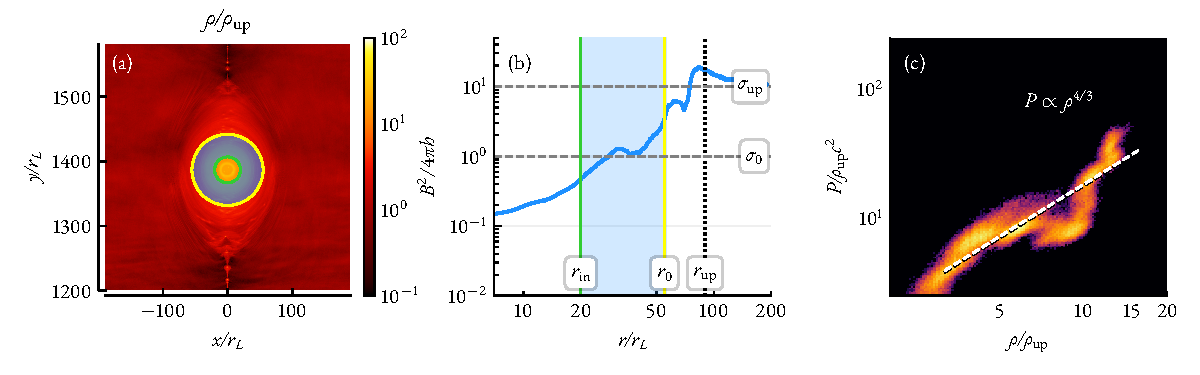
\includegraphics[width=\textwidth]{figures/ch2-reconnection/figa1_1.pdf}
    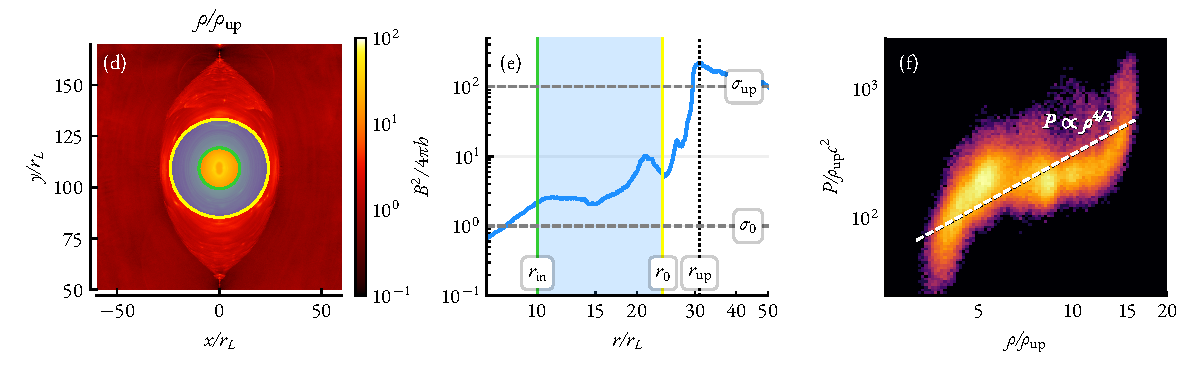
\includegraphics[width=\textwidth]{figures/ch2-reconnection/figa1_2.pdf}
    \caption{Top panels correspond to the $\sups=10$ simulation, while bottom panels are for the $\sups=100$ case. (a, d) Close-up view of an isolated primary plasmoid, with color indicating $\rho/\rho_{\rm up}$ (see color bar). The plasmoid shell, where the force balance condition \eqref{eq:rec-forcebalance} is satisfied, is shown as a blue shaded ring; the green and yellow circles indicated the core radius and the boundary of the shell. (b, e) Plasma magnetization as a function of radius from the plasmoid center (in units of $r_L$). The blue shaded region corresponds to the plasmoid shell, shown in blue in panels (a) and (d). The horizontal dashed lines correspond to the upstream magnetization, $\sups$, and the magnetization of the plasmoid shell, $\sigma_0$ (see Equation~\eqref{eq:rec-sigma0}). The three radii marked on the plot are defined in Section~\ref{sec:reconnection-plasmoids}. (c, f) Typical two-dimensional histogram of the plasma pressure and plasma density for the shaded region in panels (a) and (d). The polytropic EOS for a relativistic gas is also shown (dashed line).}
    \label{fig:rec-plasm_eos}
\end{figure}

\section{Finding the boundaries of plasmoids}
\label{appendix:rec-plasmbound}
In this section, we describe the algorithm we used for identifying the plasmoid boundaries. This relies on the mixing criterion~\citep{2014PhPl...21e2307D, 2017ApJ...850...29R} and on the vector potential.

We distinguish particles originating from one side of the current sheet, $+x$, from the ones from the other side, $-x$. Henceforth, we refer to their densities as $\rho^+$ and $\rho^-$. We then compute the so-called {\it mixing factor}, $\lambda_f$, in each cell of our simulation domain

\begin{equation}
    \lambda_f = 1 - \left(1 - 2\frac{\rho^+}{\rho^+ + \rho^-}\right)^2.
    \label{eq:rec-mixingf}
\end{equation}

The mixing factor is defined in a way that $\lambda_f = 1$ inside the plasmoids and the current sheet, where particles from two separated regions are perfectly ``mixed,'' and $\lambda_f = 0$ everywhere else. At the plasmoid edges the mixing factor takes intermediate values, $0 < \lambda_f < 1$ (see Figure~\ref{fig:rec-plasmbound}(b)). We compute the isocontours of the vector potential $A_z$ (the simulation is done in the $x$-$y$ plane). To identify the boundary of a particular plasmoid, we select regions characterized by intermediate values of the mixing factor (i.e.,  $0.1 < \lambda_f < 0.9$) and find the average value of the vector potential values in these regions, $A_z^0$. We then define the isocontour of $A_z=A_z^0$ as the boundary for that particular plasmoid (see Figure~\ref{fig:rec-plasmbound}(a), thick white line).

\begin{figure}[!ht]
    \centering
    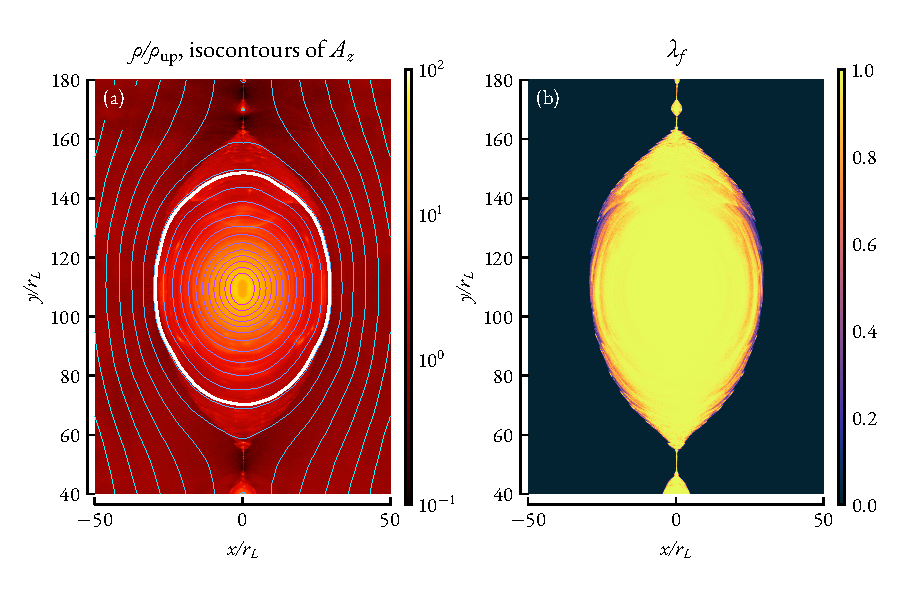
\includegraphics[width=\textwidth]{figures/ch2-reconnection/figb1.pdf}
    \caption{Zoom in of a small region of the reconnection layer (from the $\sups=100$ simulation) containing an isolated large plasmoid. Panel (a) Plasma density in logarithmic scale (see color bar on the side)  with overlaid contours of the vector potential (solid cyan lines). The thick white line corresponds to $A_z=A_z^0$ and marks the plasmoid boundary. (b) Mixing factor, $\lambda_f$, defined by Equation~\ref{eq:rec-mixingf}. The transition from $\lambda_f=1$ (fully mixed) to 0 (not mixed) happens over only a few skin depths.}    
    \label{fig:rec-plasmbound}
\end{figure}

Our results are robust to the choice of the exact mixing factor values, as $\lambda_f$ has a very steep spatial profile at the plasmoid edges; it changes quickly from $0$ to $1$ going from the upstream to the plasmoid within a few skin depths, meaning that the mixing of particles happens very abruptly. Even if one argues that our method does not yield the exact plasmoid boundary, this does not affect our results, because our analysis focuses on long-term processes taking place well within the plasmoid boundary.
